% all-in-one cheatsheet layout (Michael Franzen, 2013)
\documentclass[a4paper]{article}

% geometry settings
\usepackage[top=2cm, bottom=2.5cm, left=2cm, right=2cm]{geometry}

% font settings
%\usepackage[light,math]{kurier}
\usepackage[T1]{fontenc}
\usepackage[utf8]{inputenc}
\usepackage{marvosym}
\usepackage{amssymb}
\usepackage{amsfonts}
\usepackage{amsmath}
\usepackage{amsthm}

% colors
\usepackage{xcolor}
\definecolor{lightgray}{gray}{0.8}

% formatting
\usepackage{paralist}
\usepackage{multicol}
\usepackage{tabularx}
\usepackage{Tabbing}
\usepackage{booktabs}
\usepackage{fancyhdr}
\usepackage{url}
\usepackage{mdframed}
\pagestyle{fancy}

% math
\usepackage{array}
\usepackage{eqnarray}
\usepackage{mathtools}

% figures
\usepackage{wrapfig}
\usepackage{subfig}

% figure modules
\usepackage{graphicx}
\usepackage{tikz}
\usetikzlibrary{positioning,calc, shapes}
\usepackage{algorithm2e}
\usepackage{verbatim}

% TOC & Glossary
\usepackage{sectsty}
\usepackage[nottoc,notlof,notlot]{tocbibind}
\usepackage[titles,subfigure]{tocloft}

% commands
\usepackage{xargs}
\usepackage{ifthen}

% head line
\fancyhf{}
\chead{Graph Theory - Sheet 2 - \today\\J. Batzill (1698622), M. Franzen (1696933), J. Labeit (1656460)}
\renewcommand{\headrulewidth}{0.4pt} %obere Trennlinie

\newcommand{\sheetnumber}{1}

% (problem number)
\surroundwithmdframed[
    hidealllines=true,
    backgroundcolor=gray!10,
    skipbelow=\baselineskip,
    skipabove=\baselineskip
]{mylemma}

\surroundwithmdframed[
	linecolor=white,
	skipbelow=\baselineskip,
	skipabove=\baselineskip
]{mytheorem}

\begin{document}
	
	\newtheorem{mytheorem}{Theorem}[section]
	\newtheorem{mylemma}{Lemma}[mytheorem]	

	\newenvironmentx*{solution}[1]{\section*{Problem #1}\addtocounter{section}{1}\setcounter{mylemma}{0}\setcounter{mytheorem}{0}}{}
	\newenvironmentx*{theorem}[1]{\begin{mytheorem}#1\begin{proof}}{\end{proof}\end{mytheorem}}
	\newenvironmentx*{lemma}[1]{\begin{mylemma}#1\begin{proof}}{\end{proof}\end{mylemma}}


	\begin{solution}{5}
		\begin{center}
			
			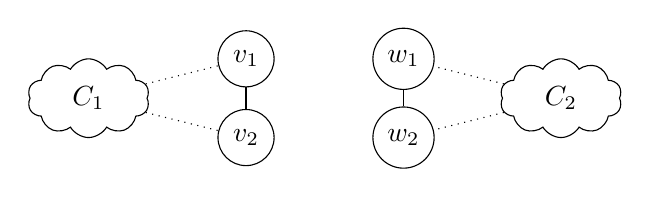
\begin{tikzpicture}
				\node[cloud, cloud puffs=10, cloud puff arc=120, aspect=2, minimum width=1.5cm, minimum height=1cm, draw] (c1)  at (-1,-0.5) {$C_1$};
				\node[circle, draw] (v1) at (1, 0) {$v_1$};
				\node[circle, draw] (v2) at (1, -1) {$v_2$};
				\draw[dotted] (c1) -- (v1);
				\draw[dotted] (c1) -- (v2);
				\draw (v1) -- (v2);

				\node[cloud, cloud puffs=10, cloud puff arc=120, aspect=2, minimum width=1.5cm, minimum height=1cm, draw] (c2)  at (5,-0.5) {$C_2$};
				\node[circle, draw] (w1) at (3, 0) {$w_1$};
				\node[circle, draw] (w2) at (3, -1) {$w_2$};
				\draw[dotted] (c2) -- (w1);
				\draw[dotted] (c2) -- (w2);
				\draw (w1) -- (w2);
			\end{tikzpicture}
		\end{center}
		\textbf{Step 1:}
		\begin{center}
			\begin{tikzpicture}
				\node[cloud, cloud puffs=10, cloud puff arc=120, aspect=2, minimum width=1.5cm, minimum height=1cm, draw] (c1)  at (-1,-0.5) {$C_1$};
				\node[circle, draw] (v1) at (1, 0) {$v_1$};
				\node[circle, draw] (v2) at (1, -1) {$v_2$};
				\draw[dotted] (c1) -- (v1);
				\draw[dotted] (c1) -- (v2);
				\draw (v1) -- (w1);

				\node[cloud, cloud puffs=10, cloud puff arc=120, aspect=2, minimum width=1.5cm, minimum height=1cm, draw] (c2)  at (5,-0.5) {$C_2$};
				\node[circle, draw] (w1) at (3, 0) {$w_1$};
				\node[circle, draw] (w2) at (3, -1) {$w_2$};
				\draw[dotted] (c2) -- (w1);
				\draw[dotted] (c2) -- (w2);
				\draw (w1) -- (w2);
			\end{tikzpicture}
		\end{center}
		\textbf{Step 2:}
		\begin{center}
			\begin{tikzpicture}
				\node[cloud, cloud puffs=10, cloud puff arc=120, aspect=2, minimum width=1.5cm, minimum height=1cm, draw] (c1)  at (-1,-0.5) {$C_1$};
				\node[circle, draw] (v1) at (1, 0) {$v_1$};
				\node[circle, draw] (v2) at (1, -1) {$v_2$};
				\draw[dotted] (c1) -- (v1);
				\draw[dotted] (c1) -- (v2);
				\draw (v1) -- (w1);

				\node[cloud, cloud puffs=10, cloud puff arc=120, aspect=2, minimum width=1.5cm, minimum height=1cm, draw] (c2)  at (5,-0.5) {$C_2$};
				\node[circle, draw] (w1) at (3, 0) {$w_1$};
				\node[circle, draw] (w2) at (3, -1) {$w_2$};
				\draw[dotted] (c2) -- (w1);
				\draw[dotted] (c2) -- (w2);
				\draw (v2) -- (w2);
			\end{tikzpicture}
		\end{center}
		\textbf{Result: } The components are connected while $d(v_1), d(v_2), d(w_1), d(w_2)$ have not been modified.
	\end{solution}
	\newpage
	\begin{solution}{6}
	In the following I will proof that any tree with a even number of vertices has exactly one spanning subgraph in which every vertex has odd degree induction. I will reduce the problem by recursively removing leaves until only the trivial case of two vertices is left. \\
	Let $T=(V, E)$ be a tree with even number. If $|V|=0$ or $|V|=2$ there is obviously exact one spanning subgraph. 
	In the following let $|V|>2$ and let $S$ be the set of edges of a spanning subgraph meeting the conditions stated above. \\
	In the lecture we proved that $T$ has atleast one leave $v$. 
	Because any leaf only has one edge $(v,u)$, this edge has to be in $S$. 
	Additionally, if the edge $(v,u)$ is part of $S$ the condition that the degree of any vertex is odd is met for the leaf $v$. 
		
	\begin{itemize}
		\item \textbf{Case 1:} There is one edge $u \in V$ connected to atleast two leaves $v_1, v_2 \in V$. \\
		We know that the edges $(u,v_1)$ and $(u,v_2)$ have to be in $S$. If we remove T
		
		\item \textbf{Case 2:} There is no edge $u \in V$ connected to atleast two leaves $v_1, v_2 \in V$. \\
		
		\begin{lemma}{In a tree $T=(V,E)$ with $|V|>2$ where there is no edge $u \in V$ connected to atleast two leaves $v_1, v_2 \in V$, there is a leaf $v \in V$ connected to a vertex $u$ with $deg(u) = 2$.}
		Proof: From the prerequisite that there is no edge $u \in V$ connected to atleast two leaves, we know that all leaves are connected to different vertices. 
		Let's assume there is no such vertex $u$, then all vertices $u \in V$ connected two a leaf have to have $deg(u) \neq 2$. 
		Because $T$ is connected and $|V|>2$ all $u$ have to have an edge and cannot be a leaf itself, hence for all such $u$ $deg(u) \geq 3$. 
		By removing all leaves from $T$ we get $T'$ a subgraph of $T$. By removing the leaves only the degree of all $u$ connected to a leaf are reduced be one. 
		Then for all $u$ $deg(u) \geq 2$ in the subgraph $T'$. 
		Additionally, because the degree of all other vertices is not changed and they are no leaves the degree of all vertices of the resulting graph is greater or equal 2. 
		Thus using a lemma of the lecture the result graph has to have a cycle. 
		Because $T'$ is a subgraph of $T$ this is a contradiction to $T$ being acyclic. 
		Hence, there has to be a vertex $u$ connected to a leaf with $deg(u)=2$. 		
		\end{lemma}
		
		Using the lemma we can find a leaf $v \in V$ with an edge $(v,u) \in E$ with $deg(v)=2$. 
		We know that the edge $(v,u)$ has to be in $S$. 
		Additionally, we know that the degree of $u$ in any spanning subgraph meeting the conditions has to be odd, so the second edge $(u,t)$ with $t \in V$ cannot be in $S$. 
		If we remove $u$ and $v$ from T we gain receive a tree with an even number of vertices. 
		Hence, we either $|V- \{v,u\}| \leq 2$ and we know that there is exact one spanning subgraph meeting the conditions, or we can again apply case 1 or case 2. 
	\end{itemize}	 
	
	
	\end{solution} 
	\newpage
	\begin{solution}{7}
		For a set $C = \{G_1, ..., G_n\}$ of connected components:\\
		\begin{align}
			\pi(C)&= \sum_{i = 1}^n \frac{|\{v \in V(G_i)\ |\ d(v) \text{ odd}\}|}{2}&
		\end{align}
	\end{solution} 
	\newpage
	\begin{solution}{8}
		
	\end{solution}
	
\end{document}